\documentclass[a4paper, 11pt]{article}

\usepackage{amsmath}
\usepackage{tikz}
\usepackage{parskip}
\usepackage{siunitx}
\usepackage{subcaption}
\usepackage{geometry}

\newcommand{\del}[2]{\frac{\partial #1}{\partial #2}}  % Partial derivative
\newcommand{\ddel}[2]{\frac{\partial^2 #1}{\partial #2^2}}
\newcommand{\deriv}[2]{\frac{\mathrm{d} #1}{\mathrm{d} #2}}  % Derivative
\newcommand{\dderiv}[2]{\frac{\mathrm{d}^2 #1}{\mathrm{d} #2^2}}  % Second derivative
\newcommand{\expval}[1]{\langle #1 \rangle}
\newcommand{\inner}[2]{\langle #1, #2 \rangle}

\title{The world of quantum mechanics}

\author{Thorvald Molthe Ballestad}

\begin{document}
\maketitle

\begin{abstract}
  This paper investigates simple numerical approaches to investigating the classical quanum mechanical problem of a particle in an infinite square well.
  The Schrödinger equatino is discretized and solved numericall using a central finite difference of second order.
  The sanity of such an approach is discussed by comparing to analytical results.
  Two methods of time development of a wave function is shown, expansion into eigenstates and a Crank-Nicolson scheme.
  In the Crank-Nicolson scheme Julia's built in solver for symmetric tridiagonal matricies is leveraged.
\end{abstract}

\section{Introduction}
The entire field of quantum mechanics i governed by the wave function given by the Schrödinger equation.
All systems are described by this simple formulation.
However, solving the equation is often difficult or impossible to do analytically, and thus require a numerical approach.
This paper investigates some of the most basic yet insightful systems and methods used in numerical quantum mechanics, including the finding of eigenfunctions of an infinite square well with a central barrier and time development using two different approaches.
Namely expansion into eigenstates and an iterative Crank-Nicolson scheme.

\section{Theory and method}
Quantum mechanics is based on the Schrödinger equation,
\begin{equation}\label{eq:SE}
i\hbar \del{}{t} \Psi = \hat{H} \Psi,
\end{equation}
where $\Psi$ is the wave function.
The wave function describes the probability of finding a particle at a given position at a given time, by
\begin{equation}
p(\vec{r}, t) = \left|\Psi(\vec{r}, t)\right|^2.
\end{equation}
The problem to be solved is thus normally to find the hamiltonian $\hat{H}$ and solving the Schrödinger equation.
For a time independent hamiltonian \eqref{eq:SE} can be written as \cite{assignment}
\begin{equation}\label{eq:tise}
\hat{H}\psi_n = E_n \psi_n,
\end{equation}
where $\psi_n$ are called eigenstates and $E_n$ are their energies.

One of the most simple systems one can investigate using this theory is a particle in an infinite one dimensional square well with a central barrier,
\begin{equation}
V(x) =
\begin{cases}
0 & \text{for} \quad 0 < x < L/3\\
V_0 & \text{for} \quad L/3 < x < 2L/3\\
0 & \text{for} \quad 2L/3 < x < L\\
\infty & \text{for} \quad \text{otherwise}.
\end{cases}
\end{equation}
See figure \ref{fig:potential}.
\begin{figure}[ht]
\centering
\begin{tikzpicture}
\draw[->] (0,0) -- (0, 5) node[midway, anchor=east] {$V = \infty$};
\draw[->] (9,0) -- (9, 5) node[midway, anchor=west] {$V = \infty$};
%\draw[->] (0,0) -- (9.5, 0) node[anchor=west]{x};
\draw (0,0) -- (3, 0) -- (3, 2) -- (6,2) -- (6, 0) -- (9, 0);
\node[anchor=south] at (4.5,2) {$V_0$};
\node[anchor=east] at (0, 0) {$x=0$};
\node[anchor=west] at (9, 0) {$x=L$};
\end{tikzpicture}
\caption{An infinite well with a central barrier of strength $V_0$.\label{fig:potential}}
\end{figure}
For such a particle, the hamiltonian is \cite{assignment}
\begin{equation}\label{eq:hamil}
\hat{H} = -\frac{\hbar^2}{2m} \ddel{}{x} + V(x).
\end{equation}
Furthermore, in the special case $V_0=0$, a well without a barrier, analytical solutions can be found easily, and are useful for numerical validation.
They are\cite{griffith}
\begin{equation}\label{eq:anal}
\psi_n(x) = \sqrt{2} \sin\left(n\pi x\right), \quad n = 1, 2, \dots,
\end{equation}
with energy
\begin{equation}
E_n = \frac{n^2\pi^2 \hbar^2}{2m}.
\end{equation}

Equation \eqref{eq:tise} describes an eigenproblem.
In order to solve it numerically dimensionless variable must be introduced and the hamiltonian \eqref{eq:hamil} has to be discretized.
Let $t=t_0 t'$ and $x=x_0 x'$.
Setting $x_0 = L$ and $t_0 = \frac{2mL^2}{\hbar}$ \eqref{eq:tise} reduces to
\begin{equation}\label{eq:dimlesstise}
\left[-\ddel{}{x'} + v(x') \right] \psi_n(x') = \lambda_n \psi_n,
\end{equation}
where $v(x') = t_0 V(x)/\hbar$.
Let $x'$ be discretized into $N$ points, and define $x'_k = k \Delta x'$, where $\Delta x' = 1/(N-1)$.
For the discretization the central finite difference of second order is used to approximate the second derivative in the hamiltonian
\begin{equation}
\ddel{f}{x'} \approx \frac{f(x'_{k-1}) - 2f(x'_k) + f(x'_{k+1})}{\Delta x'^2}.
\end{equation}
Writing $\psi_n$ as a column vector of $N$ elements, equation \eqref{eq:dimlesstise} thus becomes
\begin{equation}
\begin{bmatrix}
\frac{2}{\Delta x^2} + V_0 & \frac{-1}{\Delta x^2} & 0 & \\
\frac{-1}{\Delta x^2} & \frac{2}{\Delta x^2} + V_1 & \frac{-1}{\Delta x^2} & 0  \\
0 & \frac{-1}{\Delta x^2} & \frac{2}{\Delta x^2} + V_2 & \frac{-1}{\Delta x^2} & 0 & \dots\\
&0&\vdots&\ddots
\end{bmatrix}
\begin{bmatrix}
\psi_0\\
\psi_1\\
\vdots
\end{bmatrix}
=
\lambda
\begin{bmatrix}
\psi_0\\
\psi_1\\
\vdots
\end{bmatrix},
\end{equation}
where $\hat{H}$ now is a symmetric tridiagonal matrix and $V_n = V(x_n)$.



For a given barrier $V_0$ it can be shown analytically\cite{assignment} that the energies $\lambda < V_0$ are given by the zeros of the function
\begin{equation}\label{eq:zero}
f(\lambda) = e^{\kappa/3} \left[
\kappa\sin\left(\frac{k}{3}\right) + k\cos\left(\frac{k}{3}\right)
\right]^2
-
e^{-\kappa/3} \left[
\kappa\sin\left(\frac{k}{3}\right) - k\cos\left(\frac{k}{3}\right)
\right]^2.
\end{equation}
Thus, finding these zeros, one might use them to verify the results found solving the Schrödinger equation numerically.

Any initial condition $\Psi_0$ may be expanded into the eigenfunctions\cite{griffith}
\begin{equation}\label{eq:expansion}
\Psi_0 = \sum_n c_n \psi_n.
\end{equation}
It can be shown \cite{griffith} that the time evolution of an eigenfunction $\psi_n$ with energy $E_n$ is
\begin{equation}
\Psi(x, t) = \exp\left(-\frac{i E_n t}{\hbar} \right) \psi_n(x).
\end{equation}
Thus, for any inital $\Psi_0$ the time evolution is given as
\begin{equation}\label{eq:time_develop_expansion}
\Psi(x, t) = \sum_n c_n \exp\left(-\frac{i E_n t}{\hbar} \right) \psi_n(x),
\end{equation}
where $c_n$ is given by the expansion \eqref{eq:expansion}.
As the eigenfunctions are orthogonal\cite{griffith} the coefficients can be calculated using
\begin{equation}
c_n = \inner{\psi_n}{\Psi_0} = \int_0^1 \psi_n(x') \Psi_0(x') \mathrm{d}x'.
\end{equation}
The integral is approximated using the Trapezoidal rule,
\begin{equation}
\int_0^1 \mathrm{d}x f(x) = \frac{\Delta x}{2} \left[f(0) + f(1) + 2\sum_l f(l\Delta x)\right].
\end{equation}


A different approach to the time evolution of a state is the Crank-Nicolson scheme\cite{assignment}, which is given as
\begin{equation}\label{eq:crank_nicolson}
[1+\frac{i}{2} \Delta t H] \Psi(t + \Delta t) = [1 - \frac{i}{2} \Delta t H] \Psi(t).
\end{equation}
This equation can easily be solve using an optimized solver for symmetric tridiagonal matricies, here Julia's built in solver from the LinearAlgebra library is used, which in turn calls appropriate LAPACK functions like the \verb|stev| method.

\section{Results and discussion}
Firstly a system with $V_0=0$ was solved and the results compared to the analytical solutions, in order to verify the sanity of the model.
Discretizating $x$ into $N=900$ points the first 500 eigenvalues were found.
Figure \ref{fig:eigenvalues_to_anal} shows these and the analytical values.
Notice how the numerical solution performs worse for higher values of $n$.
Increasing $N$ improves this.

\begin{figure}[ht]
\centering
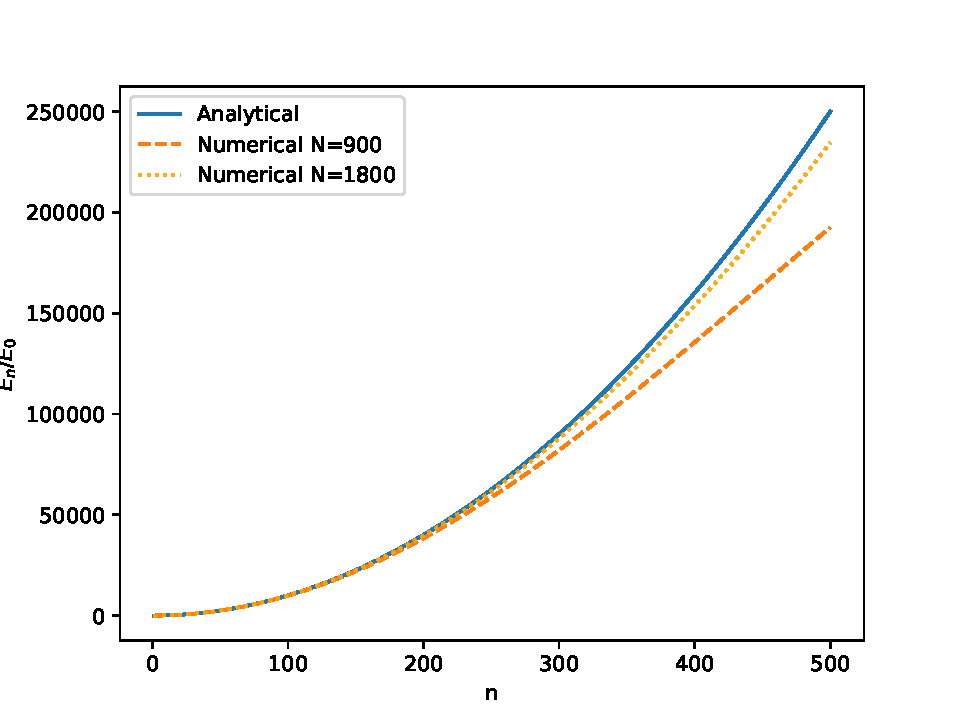
\includegraphics[width=.5\textwidth]{media/eigenvalues_error}
\caption{First 500 eigenvalues calculated for $N=900$.
Also shown is the solution calculated with $N=1800$, which is closer to the analytical results, especially for higher values of $n$.\label{fig:eigenvalues_to_anal}}
\end{figure}

For further validation of the numerical model, the eigenvalues' orthogonality was checked.
In figure \ref{fig:orthogonal} the inner product of $\psi_i$ and $\psi_j$ is shown for $i,j \in [0, 50]$ as a heatmap.
As expected, only the diagonal elements are non-zero.

\begin{figure}[ht]
\centering
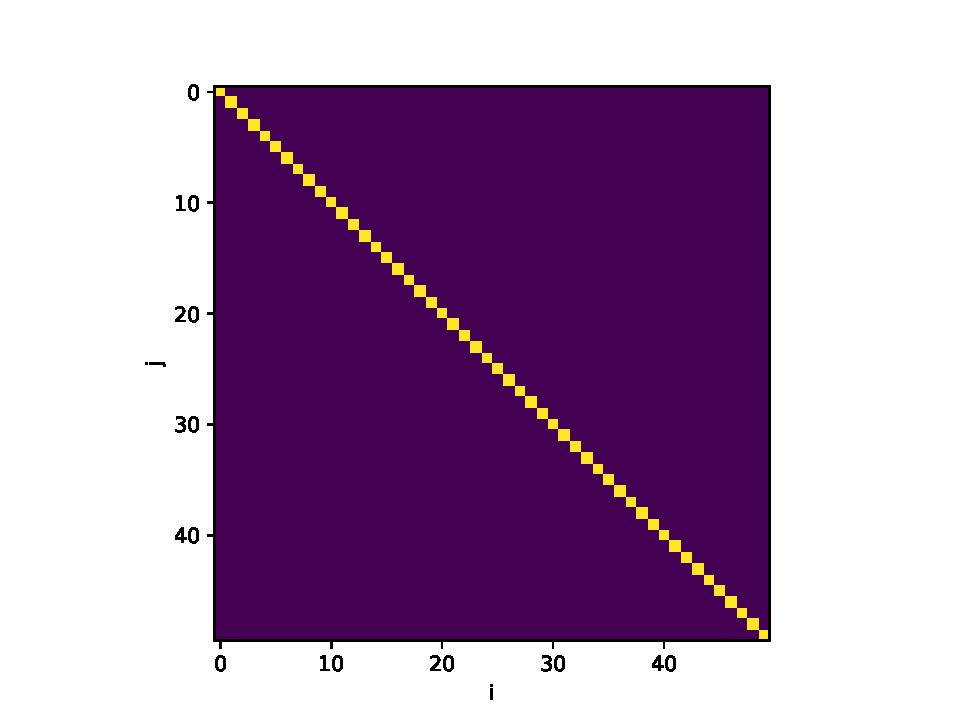
\includegraphics[width=.5\textwidth]{media/orthogonal.pdf}
\caption{The inner product $\inner{\psi_i}{\psi_j}$ for $i,j \in [0, 50]$. Only the diagonal elements, where $i=j$, are non-zero. \label{fig:orthogonal}}
\end{figure}


For a central barrier of $V_0=\num{1e3}$ the eigenfunctions are shown in figure \ref{fig:eigenfunctions}.
Notice how the eigenfunctions come in "pairs", one symmetric and one anti-symmetric, of almost the same energy.
\begin{figure}[ht]
\centering
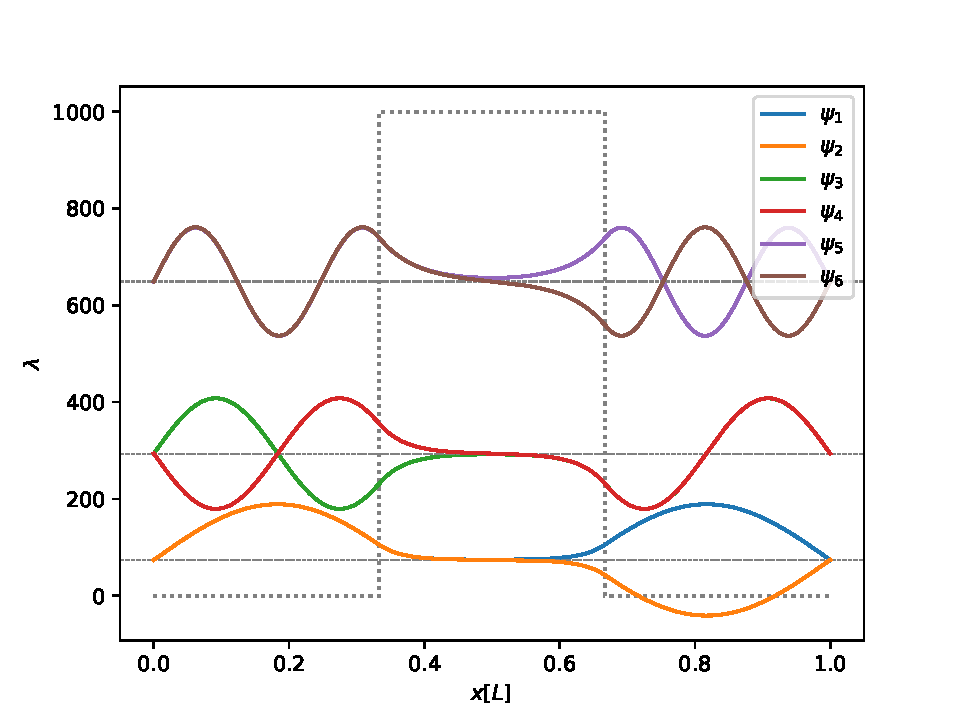
\includegraphics[width=.5\textwidth]{media/eigenfunctions}
\caption{The 6 first eigenfunctions for a system with $V_0 = \num{1e3}$. \label{fig:eigenfunctions}}
\end{figure}
The energies are given in table \ref{tab:energies}.
Also shown in the table is the ratio between the energy separation of pairs found solving the Schrödinger equation, $\lambda_{SE}$, and found by locating the zeros of \eqref{eq:zero}, $\lambda_\text{zero}$.
The calculated separations are in good correspondence with each other, with the biggest difference being at pair 1, where the ratio between them is 0.996, or equivalently a relative error of 0.4\%.

\begin{table}[ht]
\centering
\begin{tabular}{l r r l r}
Pair & $\lambda_S$ & $\lambda_{AS}$ & $\frac{\Delta \lambda_{SE}}{\lambda}$ & $\frac{\Delta \lambda_{SE}}{\Delta \lambda_{\text{zero}}}$\\
\hline
1 & 73.9724 & 73.9744 & \num{2.6009e-5} & 0.996\\
2 & 293.6354 & 293.6592 & \num{8.1060e-5} & 0.997\\
3 & 648.5636 & 648.0492 & \num{7.4819e-4} & 0.999
\end{tabular}
\caption{Energies \label{tab:energies}}
\end{table}



With $V_0 = \num{1E3}$ the superposition of the two first eigenfunctions were developed in time using the method of expanding into eigenfunctions, \eqref{eq:time_develop_expansion}, shown in figure \ref{fig:bouncy_state}.
This state has energy $\lambda \approx 74$.
Notice how the particle is first located on one side of the barrier.
It then proceeds to "move" to the other side of the barrier, even though the energy is lower than that of the barrier!
This displays tunneling -- the particle has moved through a barrier that classically would be impossible to overcome.

\begin{figure}[ht]
\centering
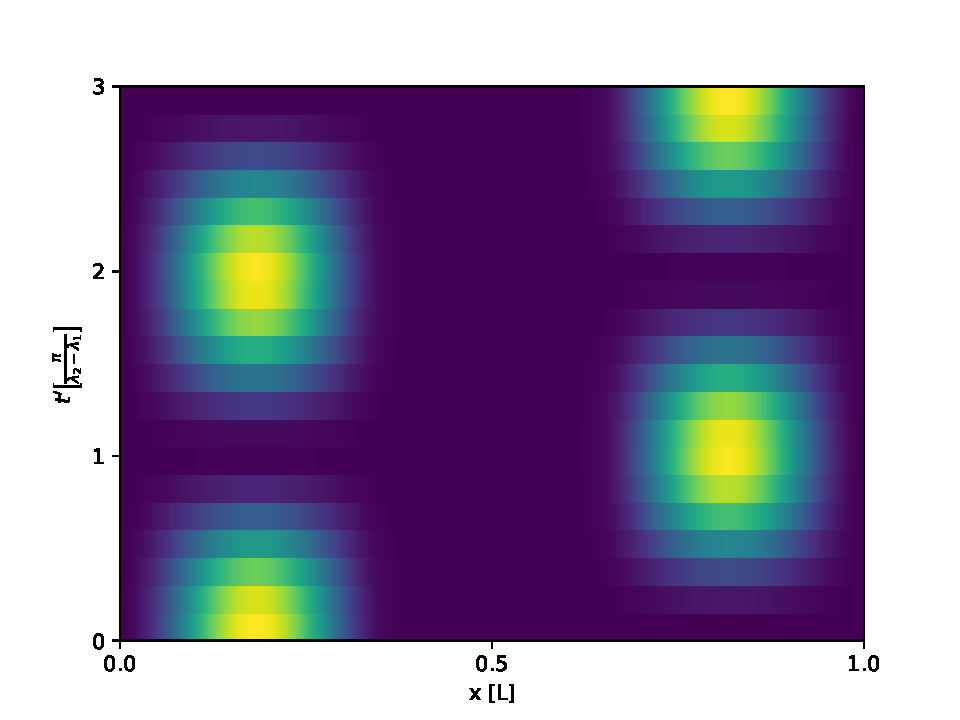
\includegraphics[width=.45\textwidth]{media/bouncy_state}
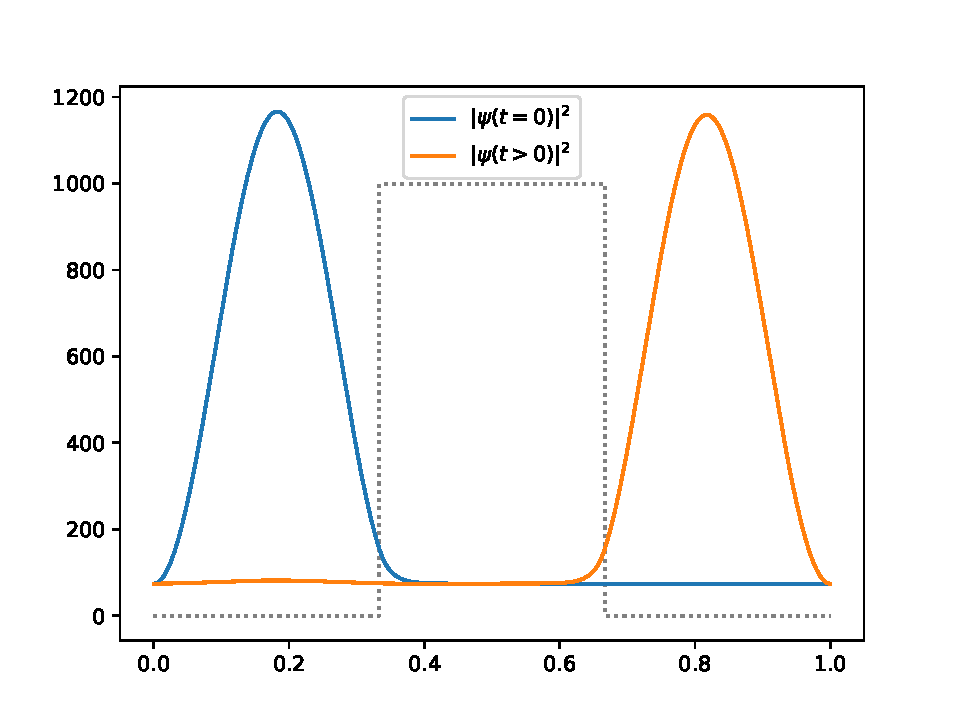
\includegraphics[width=.45\textwidth]{media/tunneling_line}
\caption{\emph{Left:} The probability function $|\psi|^2$ developed through time. Not shown is a central barrier with $v_0 = \num{1e3}$.
  \emph{Right:} The probability funtion $|\psi|^2$ shown for two different times. The dashed line is the potential function, with a central barrier of $v_0 = \num{1e3}$.
  The baseline of the wave function is the function's energy, approximately $\lambda = 74$, which is much lower than the barrier height.
  \label{fig:bouncy_state}}
\end{figure}

%% \begin{figure}[ht]
%% \centering
%% 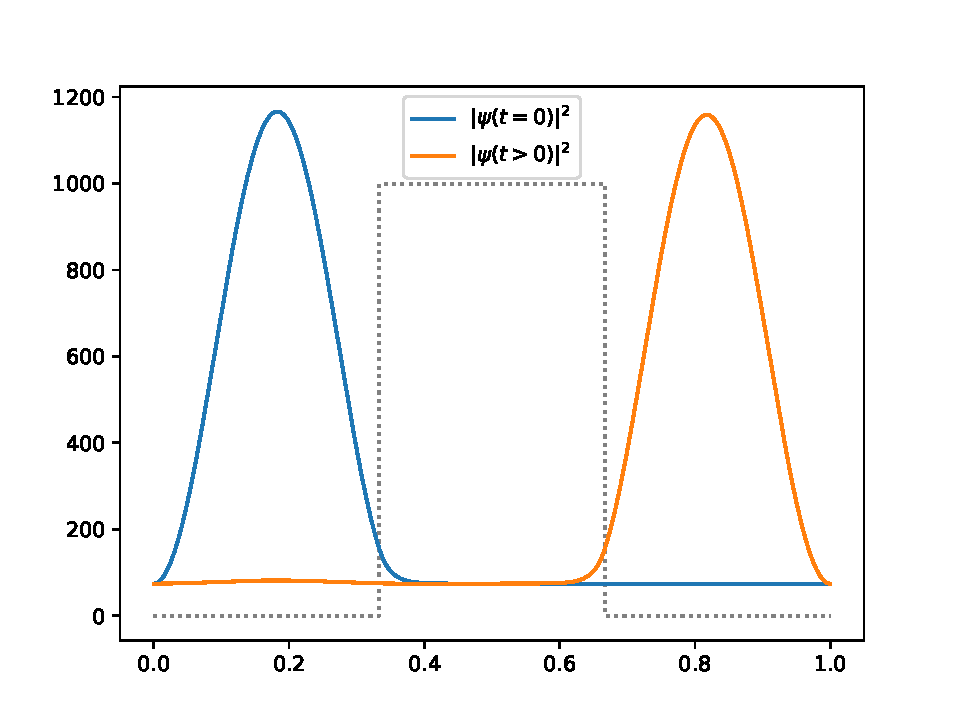
\includegraphics[width=.5\textwidth]{media/tunneling_line}
%% \caption{\label{fig:tunneling_line}}
%% \end{figure}

This method does not work for all initial states, however.
Figure \ref{fig:delta} shows a simulation with $V_0 = 0$, with the initial state being a dirac delta function $\Psi_0 = \delta(x - 1/2)$.
In the figure, the the function is shown for $t'=0.001$, and the results are obviously wrong.
As the dirac function contains waves of infinitely many moments, one would need infinitely many eigenfunction to develop using the expansion method.
For such cases, the Crank-Nicolson method might be better, as it does not require expansion into eigenstates.
The downside of an iterative method, however, is that it requires much computiational time to simulate for big time scales, as was done in the tunneling example.
Note to self: hvis dette blir innlevering, så legg inn et eksempel på noe gjort med crank-nicolson her.
\begin{figure}[ht]
\centering
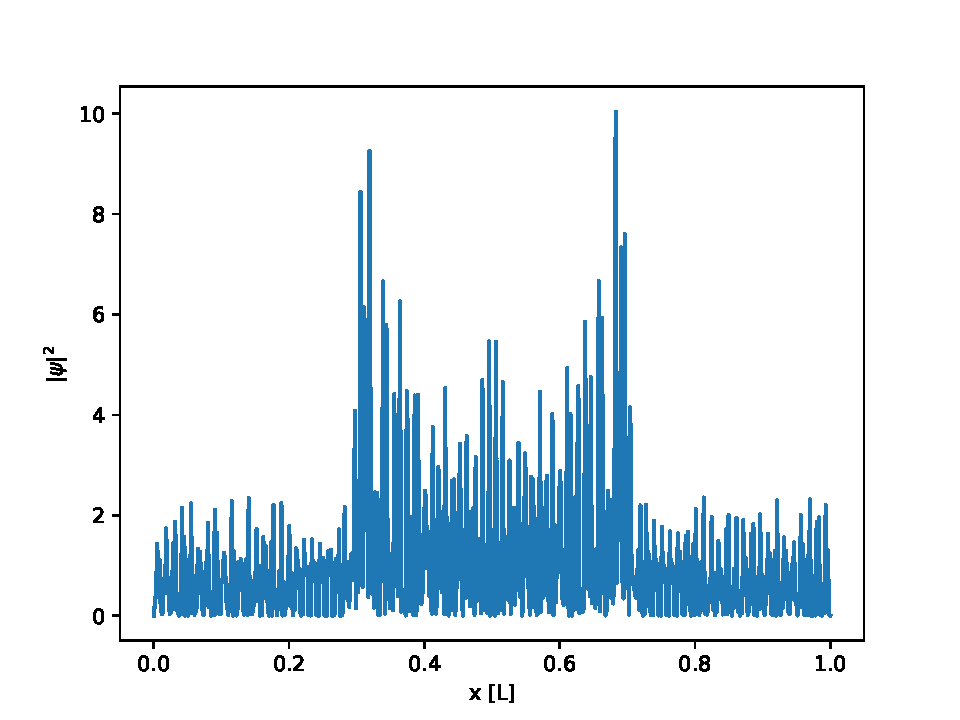
\includegraphics[width=.5\textwidth]{media/delta}
\caption{A dirac delta function developed to time $t'=0.001$ using the method expansion to eigenfunctions. \label{fig:delta}}
\end{figure}

\section{Conclusion}
Using only very simple numerical methods one is able to find interesting quantum mechanical results, such as the tunneling effect.
The eigenvalues that are found are also very precise, here with only 0.4\% relative error in the $v_0 = \num{1e3}$ system.
A continuation of this work would be more rigorous investigation of error, especially in the time development.
For example, future work should investigate the difference in results with a Crank-Nicolson simulation from the expansion method.
This should especially be considered with regards to how the initial condition is able to expand into the eigenstates.
If the inital state is well localized in momentum-space, requiering few eigenfunctions to represent, the results from an expansion solution should perform well, as it did in this report.
However, how the expansion method and Crank-Nicolson method performs for non-localized inital states in momentum-space requires more investigation.

\begin{thebibliography}{9}
\bibitem{assignment} Assignment
\bibitem{griffith} Griffith
\end{thebibliography}
\end{document}
